\chapter{An Introduction to Knotted Fields}

\section{Kelvin's vortex atom}
\label{sec:Kelvin}
The original, and perhaps most familiar, example of a knotted field is the smoke ring. Easily made by cutting a circular hole in a rectangular box, then replacing the opposite side entirely with a sheet of rubber, ``a blow on this flexible side causes a circular vortex ring to shoot out from the hole on the other side'' \citep{Kelvin}. In 1867, exactly this demonstration was shown to Lord Kelvin by Peter Guthrie Tait. What is generated is a tightly circulating tube of air, closed into a ring, which propagates stably across the room, rebounding elastically from walls and even other vortex rings (of course to see the ring one first needs to fill the box with smoke, perhaps using dry ice or ``a small quantity of muriatic acid'' \citep{Kelvin}). At the time, the microscopic nature of atoms was still under debate, and the stability of the rings, a consquence of Helmholtz's laws of vortex motion in an ideal fluid \citep{Helmholtz} (translated into English by Tait), coupled with their elasticity and capacity for internal vibration \citep{KelvinMasters, KelvinAMS} prompted Kelvin to suggest that ``Helmholtz's rings are the only true atoms". Kelvin hypothesised that such rings, embedded in a ``perfect homogenous liquid''\footnote{Kelvin did not actually specify whether this fluid was the same as the `ether' hypothesised to transmit electromagnetic waves \citep{KelvinMasters}.}, and ``linked together or ...knotted in any manner'' might form the microscopic basis of all matter \citep{Kelvin}.
\begin{figure}[htbp]
\centering
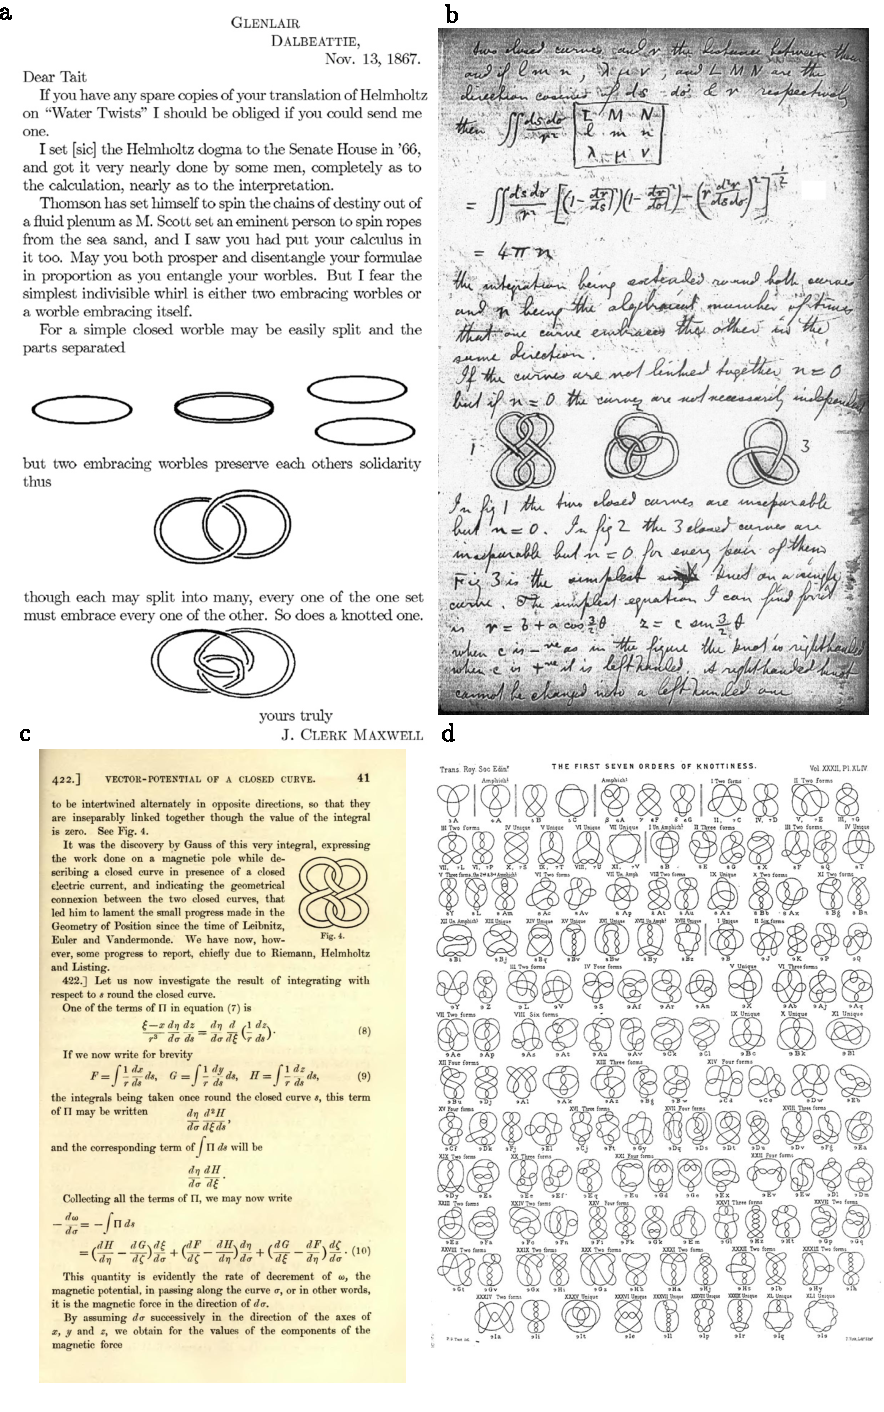
\includegraphics[width=0.99\linewidth]{\IntroductionFigures/History.pdf}
\caption{hi }
\label{fig:History}
\end{figure}

Kelvin's ``vortex atom'' rapidly encountered difficulties in its mathematical content, its falsifiability, and a lack of contempory experimental support \citep{KelvinMasters}. However its content, summarised as ``\textit{Physics = Geometry}'' in Ref. \citep{KelvinAMS}, was compelling (perhaps slightly dangerously so) and apparently motivated Tait, in ``consideration of the forms of knots by Sir W. Thomson's (Lord Kelvin) Theory of Vortex Atoms'', to construct the first systematic tables of knots in 1876--1885 (Figure \ref{fig:History}) \citep{Tait1, Tait2, Tait3}. Tait's articles, alongside a ``very remarkable essay by Listing ... and an acute remark made by Gauss ... with some comments on it by Clerk-Maxwell'' \citep{Tait}form the initial studies in  what is now the mathematical field of Knot Theory \cite{Lickorish}. Maxwell himself, although not an active contributor to vortex atom theory, had a clear interest in the ideas, encouraging Tait and Kelvin to ``prosper and disentangle your formulae in proportion as you entangle your worbles'' (Figure \ref{fig:History}) \citep{MaxwellTaitLetter}. Indeed the ``comments by Clerk-Maxwell'' referred to by Tait are in fact Maxwell's rederivation of Gauss's Linking number, as presented in his \textit{Treatise on Electricity and Magnetsim} in 1873, about which we will have much more to say in \ref{ch2}. 

Despite forming the starting point for modern knot theory, the knotted structures above are quite different to those found in your shoelaces, or in the world of art and design outside the physics department\footnote{or so I am told.}. Rather than a single knotted curve, we have a continuous fluid in whose structure the knot is encoded, and from which dynamical properties of the knot (its motion, stability, a spectrum of vibrational modes etc.) may be derived. More precisely, we have a concentrated tube of vorticity in the fluid, tied into the shape of a knot. Helmholtz's laws of vortex motion demonstrated that, in a perfect (frictionless) fluid this tube of vorticity was `frozen in' to the fluid, unable to dissapate or cross itself. In an idealised vortex atom, the radius of this tube would tend to zero, with the vorticity contained inside becoming infinite, and we would have a singular linelike structure, tied into a knot and embedded into a continuous three dimensional medium. A structure of this general form is called a \emph{knotted field}, of which the vortex atom may be considered a prototype; as we shall see, such structures are not just confined to fluids. 

The disconnect between a knotted curve and a knotted field is reflected in Tait's work, which mentions Kelvin's Vortex Atoms briefly as motivation, but focuses in substance on ``\emph{the investigation of the essentially different modes of joining points in a plane}'' \citep{Tait1}. As knot theory developed, its initial connections to hydrodynamics and electromagnetism were further abandoned. We also note that despite the wonderful knot tables produced by Tait (figure \ref{fig:History}) and the reliance of vortex atom theory on knotted and linked vortices, there is no mention above of any experimental evidence on vortices tied in nontrivial knots. 

\section{Modern knotted fields: experiments}
\subsection{Experiments in fluids}
\begin{figure}[htbp]
\centering
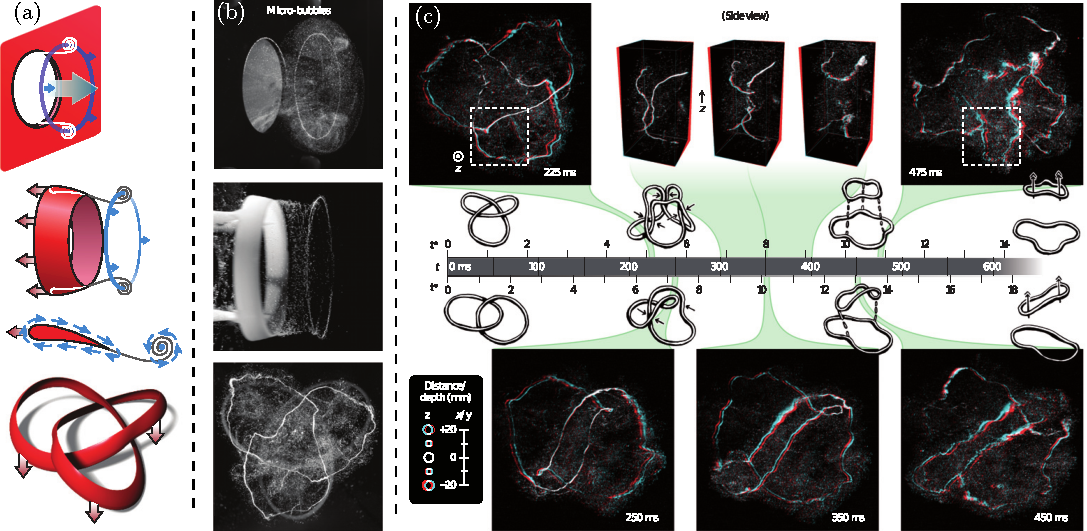
\includegraphics[width=1 \linewidth]{\IntroductionFigures/Irvine_Figs1_3.pdf}
\caption{hi }
\label{fig:Irvine}
\end{figure}
The first experimental construction of nontrivial knotted fluid vortices came 140 years after their initial theoretical investigation, from the Irvine lab in 2013 --- we show in figure \ref{fig:Irvine} several remarkable figures reproduced from Ref.~\citep{Kleckner2013}, in which Kleckner et al. tied a single vortex in water into a trefoil knot, the simplest nontrivial knot, as well as linking two of them together (Kelvin's proposed model for a Sodium atom), before tracking their evolution in full 3D. We postpone a theoretical discussion until \ref{sec:}, but note immeadiately that in a real fluid vortices do not behave like Kelvin's vortex atoms. They are not stable, but rather undergo a series of strand reconnections resulting in multiple disconnected unknots.

Ref.~\citep{Kleckner2013} is a noteable example of a more general trend; over the past $\sim10$ years knotted fields have gone from being purely theoretical constructions to being experimentally realisable in a number of systems, and though originally concieved of in fluid dynamics, modern applications are not limited to this context; they have been realised as nodal lines of optical beams~\cite{Dennis2010} and as disclinations in nematic liquid crystals and spinor Bose-Einstein condensates~\cite{Tkalec2011,Tasinkevych2014,Copar2015}. The liquid crystal system in particular is a primary motivator for this thesis, and in \ref{ch:3} we will discuss knotted fields in a novel form of liquid crystal~\cite{LavrentovichReview}, so it is worth giving a detailed description of the experiment; it also provides a second example of a knotted field not arising from hydrodynamics, which we can compare and contrast with the hydrodynamical case.

\subsection{Experiments in liquid crystals}

\begin{figure}[htbp]
\centering
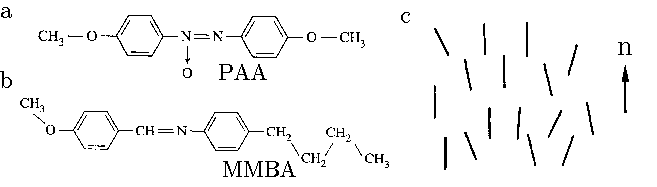
\includegraphics[width=1\linewidth]{\IntroductionFigures/DeGennesMontage.pdf}
\caption{hi }
\label{fig:DeGennesMontage}
\end{figure}

Liquid crystals are a class of materials which possess properties associated to both liquids and solids. In their most common form, the nematic phase, they show no positional order, and flow like a liquid \cite{DeGennes}. However, they do show orientational order: if one attempts to twist a portion of the liquid crystal it will respond elastically, as a solid would\footnote{This is remarkable: imagine your surprise if, upon attempting to stir your coffee, you found it fiercly resisted your attempts to turn the spoon, but was nevertheless happy to be poured down the sink.}. The molecules which comprise nematics, two examples of which are shown in Figure \ref{fig:DeGennesMontage}, are typically thin rods which align themselves along some common axis. In continuum theories this orientational order is described by a spatially varying unit vector field $\bf n$, called the director, which represents an average local molecular orientation, as shown in Figure \ref{fig:DeGennesMontage} (c). For our purposes, the most interesting thing about this order is where it breaks down; a celebrated feature of liquid crystals are their topological defects, places in the material where the director is undefined. These defects may be easily seen in a 2D slice of nematic placed between cross polarisers, creating a Schlieren texture \cite{DeGennes} like the one shown in figure \ref{fig:Disclination}(e). Places in the sample where the director is aligned with one of the two shown polarizer directions H and V will not transmit light, leading to the dark brushes observed. At points where these brushes meet, we cannot define the director; these are the defects. Note immeadiately that some defects have four brushes entering them, some only have two. Traversing a circle around a defect with two brushes, the director is aligned with each of H and V only once; in other word it makes only half a turn in a full circle around the defect. This observation is enough to establish that the director $\bf{n}$ must in fact be non-orientable; it should not be thought of as a vector field, but as a line field, for which $\bf n \sim - \bf n$. In figure \ref{fig:Disclination} (a)--(d) we show configurations of the director around these defects, with their associated Schlieren texture brushes. In (a) and (d) we have four brushes, and a line field which can be oriented; to emphasise this fact we have decorated the line field with one of the two possible choices of arrowheads. Figures (b) and (c) correspond to the non-orientable two brush case; here one cannot consistently assign arrowheads to the rods (it is worth trying to imagine doing so). In two dimensions these defects, also called disclinations or dis\emph{in}clinations \cite{Frank}, are points, but in three dimensions they are lines, transverse cross sections of which have local profiles resembling the two dimensional case; a schematic illustration is shown in Figure \ref{fig:Disclination}(f). 
\begin{figure}[htbp]
\centering
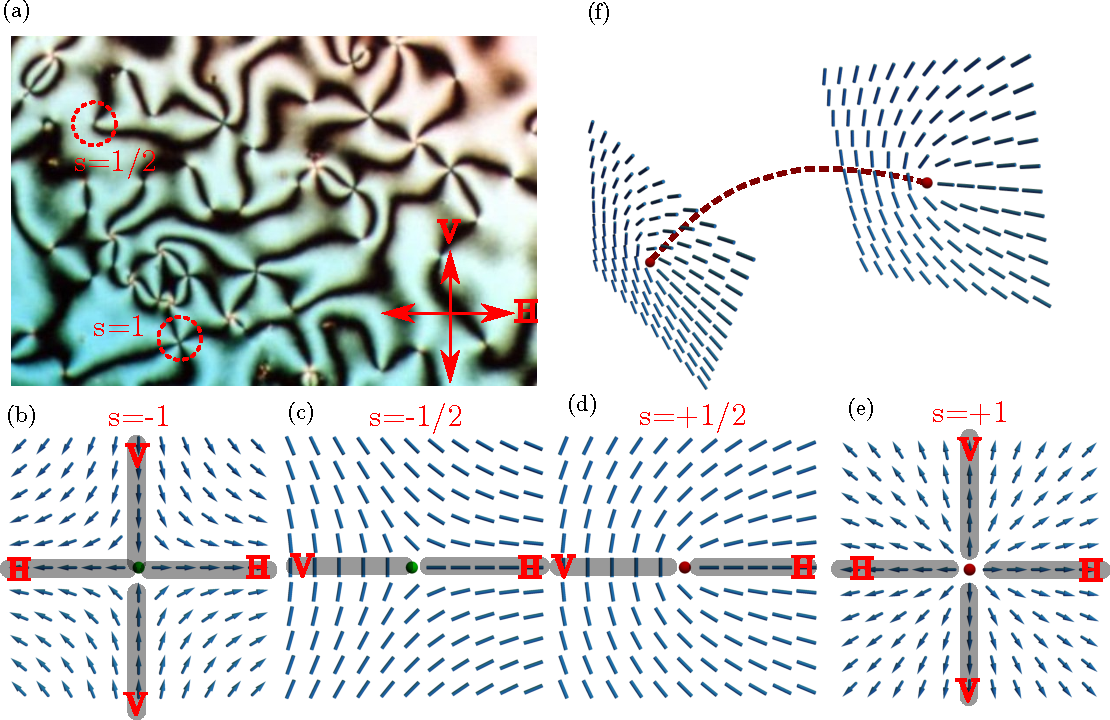
\includegraphics[width=1\linewidth]{\IntroductionFigures/DisclinationLine.pdf}
\caption{hi }
\label{fig:Disclination}
\end{figure}

One of the major advantages of working with liquid crystal disclinations is the fine control experimentalists have over them. The disclinations shrink under line tension \cite{Tkalec2011} acting as microscopic rubber bands, and may be manipulated using lazer tweezers. In order to stabilise against contraction, Refs.~\cite{Tkalec2011,Tasinkevych2014,Copar2015} wrap them around colloidal inclusions of diameter $4.72$ $\mu$m within a 5.5 $\mu$m thick slab of liquid crystal; Figure \ref{fig:KnottedLiquidCrystal} shows an example of the lazer tweezer manipulation of these `Saturn's rings'. Remarkably, when two of these colloids are brought together, the disclinations, either spontaneously or induced by the tweezers, fuse together. Assembling an array of these colloids as in \ref{fig:KnottedLiquidCrystal)} (b) and weaving the disclination lines around them, this setup allows targeted construction of certain knotted and linked tangles; examples of some possible link topologies are shown in Figure \ref{fig:KnottedLiquidCrystal} (b). This system also illustrates that knotted fields have more structure than a single knotted curve; the curve organises the entire field  (in this case the director $\bf n$) around it. Figure \ref{fig:KnottedLiquidCrystal}(c) shows a colloidal tangle under a $\lambda$ plate, which allows one to distinguish regions where the director $\bf n$ is twisting in either a right or left handed sense by the colouring of the image. We see that the disclinations separate regions of the liquid crystal into alternately right and left handed regions. This division allows construction of a surface spanning the disclinations, called the Pontryagin-Thom (PT) surface \cite{Chen}, which classifies the topology of this liquid crystal texture; for any fixed knotted disclination, there may in fact be several director configurations which cannot be deformed continuously into one another \cite{Machon}, and the PT surface detects this. 

We have now seen two examples of knotted fields in different systems and may already note some general features. The first is that the nature of the field supporting the knot may differ between systems: In that of Ref. \cite{Klecker2013}, it is the fluid velocity, a vector field. In the system of Refs.~\cite{Tkalec2011,Tasinkevych2014,Copar2015} it is the line field $\bf n$. The second is that the dynamics of the knotted fields differ dramatically between the two systems. In the first they are governed by the Navier-Stokes equations of fluid flow, where fluid viscosity causes the knot to suffer reconnections. In fact, even in the absence of viscosity (under the  Euler equations governing Kelvin's atoms), it is unclear if stable forms actually exist for knotted vortices \cite{Kida}. By contrast knot dynamics in Refs.~\cite{Tkalec2011,Tasinkevych2014,Copar2015} are governed by minimisation of the appropriate free energy for the system \cite{DeGennes, Frank}, which causes disclination lines to shrink under line tension unless stabilised (here by the colloidal inclusions). 

This thesis is primarily about Soft Matter systems, and these experiments also provide an answer to the question ``why Soft Matter?''. Soft Matter systems may be loosely chareceterised as those for which geometry plays a fundamental role in their description, and which may undergo substantial deformations in reponse to external forces, changes in temperature etc. The two systems described above, fluids and liquid crystals, are prime examples. Such systems have several appealing features. As we have seen, they are often experimentally accessible, and within the world of soft matter we find a rich diversity of types of order. For example, Refs.~\cite{Tkalec2011,Tasinkevych2014,Copar2015} use the simplest mesophase of liquid crystal, the nematic, however many other types of order are possible \cite{DeGennes}: in \ref{ch3} we study a recently discovered phase, the Twist-Bend nematic \cite{Lavrentovich}, comprised of banana-shaped molcules (in contrast to the rodlike mocules of Figure \ref{fig:LiquidCrystals}). They are described by the director $\bf n$ as in the nematic, but additionally a vector field $\bf p$ describing the local bending of the molecules. As one might expect, this second field $\bf p$ leads to topological features not present in the nematic phase. A more practical motivator, the accessibility of these systems make them candidates for industrial application \cite{Musevic}: witness the ubiquity of Liquid Crystal Display (LCD) screens.

\begin{figure}[htbp]
\centering
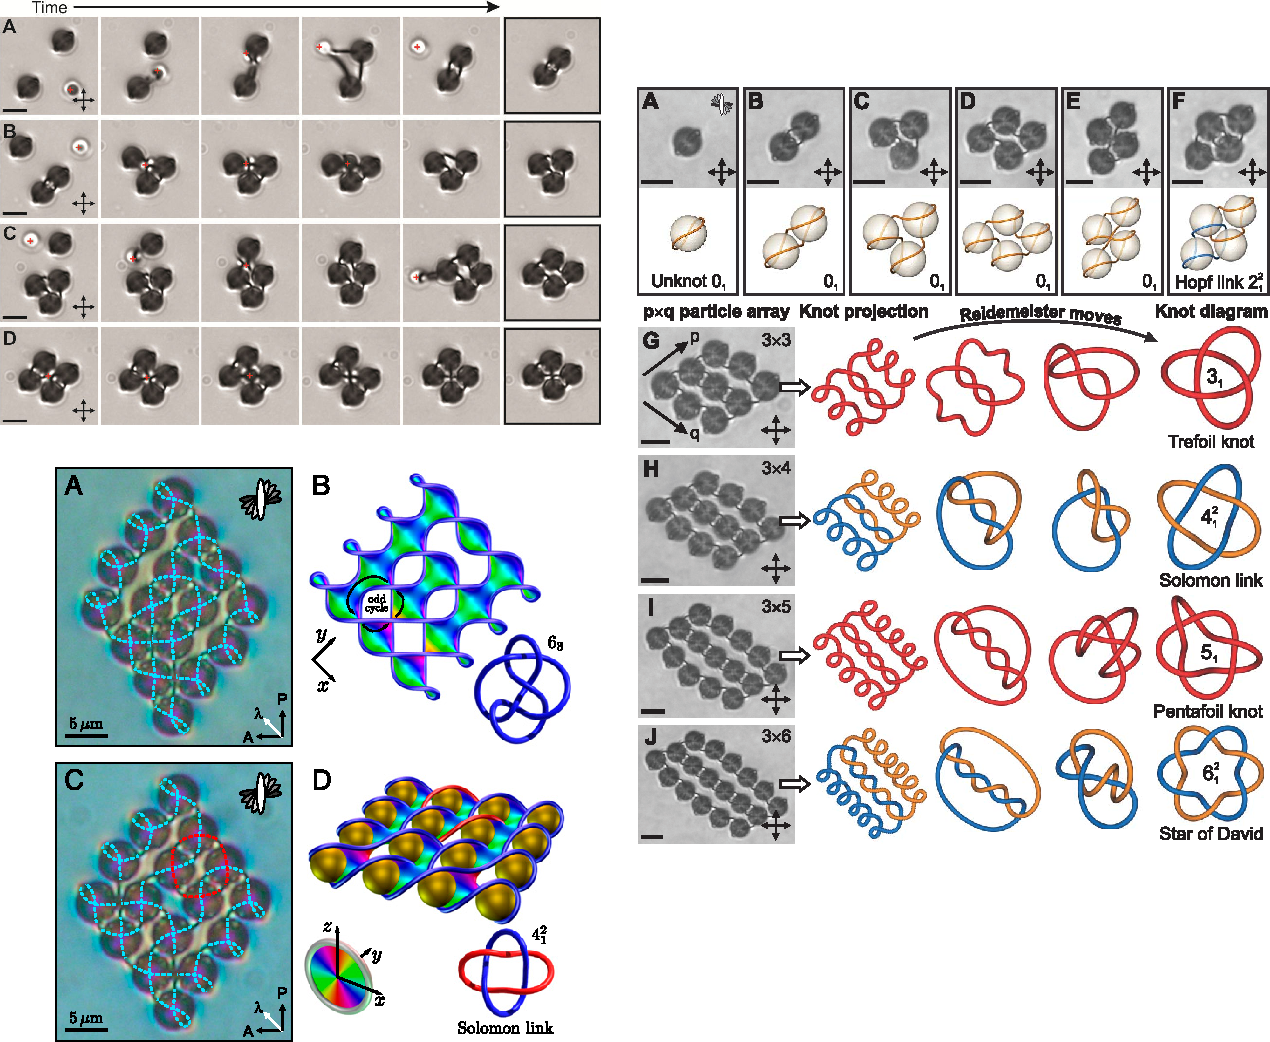
\includegraphics[width=1 \linewidth]{\IntroductionFigures/LiquidCrystalMontage.pdf}
\caption{hi }
\label{fig:KnottedLiquidCrystal}
\end{figure}

\section{Modern knotted fields: theory and simulation}
\subsection{Helicity, fluids, superfluids}
With the decline of Kelvin's vortex atom theory and the development of knot theory away from its hydrodynamic origins, a resurgence of interest in knotted fields might be dated to 1958-1969,with Moreau and Moffat's seminal papers on Helicity in ideal fluids \cite{Moreau,Moffat}, preceded by analogous results in magnetohydrodynaimcs by Woltjer \cite{Woltjer}. Focusing on the ideal fluid, both Moreau and Moffat independently demonstrated that the Helicity

\begin{equation}
    \mathcal{H} = \int {\bf u} \cdot {\bf \omega} \ d^3 \bf r,
\end{equation}
where $u(\bf r,t)$ is the fluid velocity and $\omega = \nabla \times \bf u$ is the vorticity \cite{Saffman}, is conserved under the Euler equations of ideal flow. Moffat in particular gave this invariant a topological interpretation: it measures the linking of vortex tubes within the fluid. Given a fluid where $\omega$ is concentrated along discrete sets of curves $C_i$, Moffat showed that:

\begin{equation}
    \mathcal{H} = 2 \sum_{i,j} Lk(C_i,C_j) \Gamma_i \Gamma_j 
\end{equation}
Where $\Gamma_i$ is the vorticity flux of along curve $C_i$, and $Lk(C_i,C_j)$ is the Gauss Linking number between curves $C_i, C_j$ (this interpretation of Helicity actually extends to the case where the vorticity is not concentrated along a finite set of curves, but is distributed throughout the fluid \cite{Arnold,Berger,Berger}). Figure \ref{fig:Moffat} shows several examples of vortex tubes with different linking numbers and hence helicities. Seen in this light, the conservation of Helicity is a direct consequence of Helmholtz's laws of vortex motion, and is equivalent to the statement that initially linked vortex tubes remain so; in some sense it is remarkable that the result was not known to Kelvin and Maxwell.
\begin{figure}[htbp]
\centering
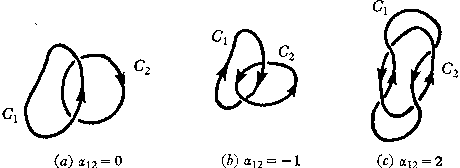
\includegraphics[width=1 \linewidth]{\IntroductionFigures/Moffat.pdf}
\caption{hi }
\label{fig:Moffat}
\end{figure}

When vorticity is not concentrated along a singular curve but distributed in a thin vortex tube, there is additional internal structure --- one imagines a knotted ribbon (Figure \ref{fig:RibbonMontage}(b)), or rubber bicycle tyre (Figure \ref{fig:RibbonMontage}(a)). Flux lines may wind around the centre-line of this tube as in Figure \ref{fig:RibbonMontage}(a), endowing it with a second linking number, the Self-Linking number, which measures the linking of any flux line with the curve centre-line, or equivalently the number of rotations any flux line makes as we traverse the centre-line once. 
\begin{figure}[htbp]
\centering
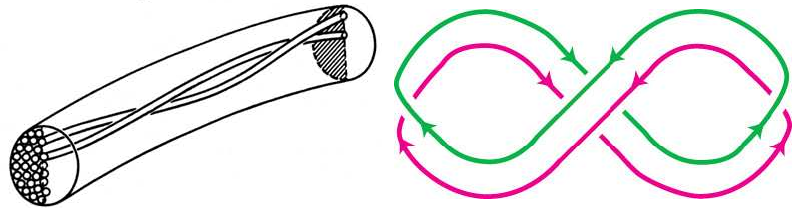
\includegraphics[width=\linewidth]{\IntroductionFigures/RibbonMontage.pdf}
\caption{hi }
\label{fig:RibbonMontage}
\end{figure}
Incorporating this structure into the helicity we find \cite{MoffatRicca}
\begin{equation}
    \mathcal{H} = 2\sum_{i,j} Lk(C_i,C_j) \Gamma_i \Gamma_j + \sum_{i} \Gamma_i^2 SL(C_i) 
    \label{eq:HelicityCount}
\end{equation}
where $SL(C_i)$ denotes the self linking of each curve $C_i$ with its implicitly assumed ribbon. In a real (viscous) fluid, helicity is not \emph{a priori} conserved. The question of whether it is in practice, and the mechanism of its dissipation, are areas of active research and motivation for the experiments shown in Figure \ref{fig:Irvine} \cite{Klecker}. 

The hydrodynamic (and magnetohydrodynamic) story of knotted fields is well developed. We have given a sketch, but the reader is invited to find more detail in reviews such as Refs. \cite{Moffat, Irvine}. The point, however, is that the above discussion acts as a template for what one might expect in knotted fields more generally. Linking, self-linking, and their connection to conserved quantites in analogy to (\ref{eq:HelicityCount}) occur in a variety of contexts \cite{Winfree}; we will meet a result of the same structure in our study of twist-bend nematics in \S \ref{ch:3}. For example, one particularly close cousin of the situation in fluids is that of superfluids, described by a complex scalar field $\psi = |\psi| e^{i \phi}$ (Figure \ref{fig:SuperFluidMontage}(a)) evolving via the non-linear Schroedinger equation \cite{}. Here vortices are given by singular lines where the circle-valued phase field $\phi$ is undefined, and about which it winds by $2\pi$. As in fluids, one may define some notion of helicity (although its precise form is more ambiguous than is the case in fluids \cite{Salman}), initialise knotted vortices and study their evolution (figure \ref{fig:SuperFluidMontage}(b)) \cite{Scheeler}. The helicity evolution turns out to be remarkably similar to that in real fluids \cite{Scheeler}. Coupled to this observation, it is found that superfluid knots also spontaneously untie over time, an example of which is shown in Figure \ref{fig:SuperFluidMontage}(b). Again, the mechanism of untying is a subject of active research \cite{Scheeler}.
\begin{figure}[htbp]
\centering
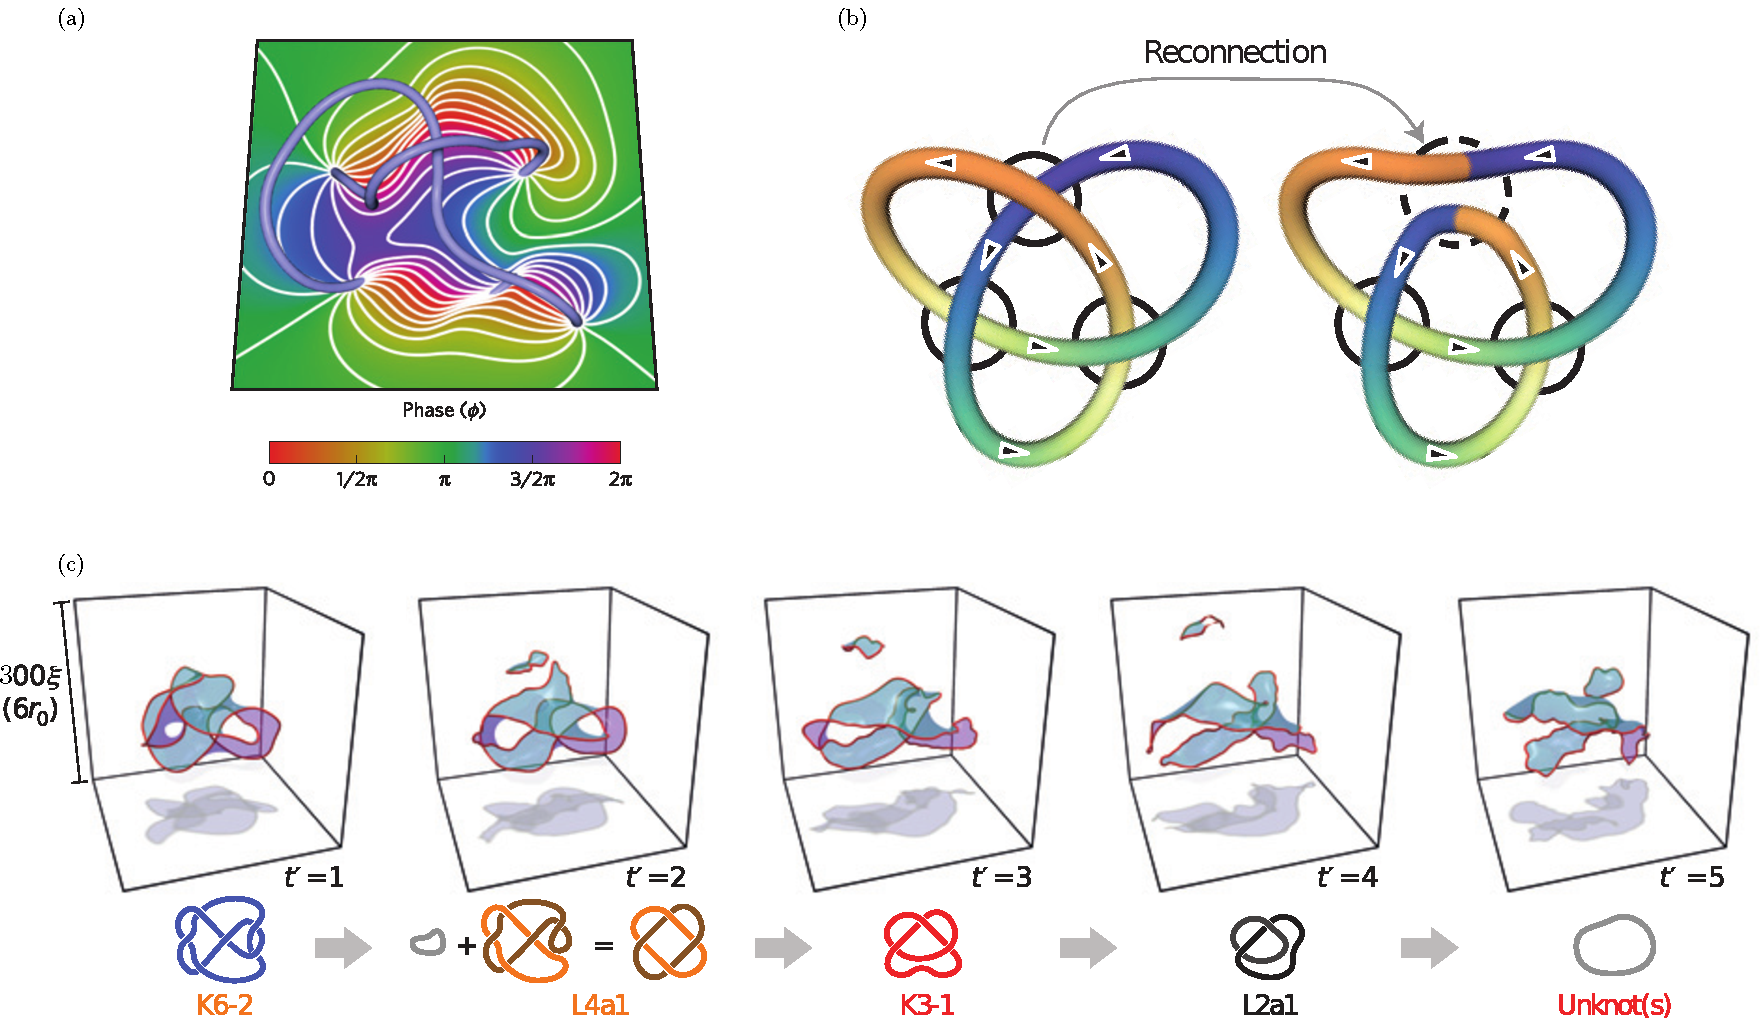
\includegraphics[width=\linewidth]{\IntroductionFigures/SuperFluidsMontage.pdf}
\caption{hi }
\label{fig:SuperFluidMontage}
\end{figure}
\subsection{Liquid Crystals and Algebraic Topology}
We now turn to a quite different, more recent line of work.

Tom,Gareth: disclinations, PT surfaces, Umbilics

\subsection{Excitable Media}

\section{Topology}

% DYNAMICS !?
% pt surface, toms classification! copar etc.
% SUPERFLUIDS - Kleckner ,untying etc.
% optical nodal beams, EM.

%For example, note immeadiately that the nematic disclination line in Figure\ref{fig:Disclination}(f) shows internal structure capable of self linking.

% Moffat
% Berger 
% Dennis Berry
% Kleckner
% Arnold
% Sutcliffe
%Winfree,Maucher
